\section{Method: \methodname}
\label{sec:method}
\begin{figure}
    \centering
    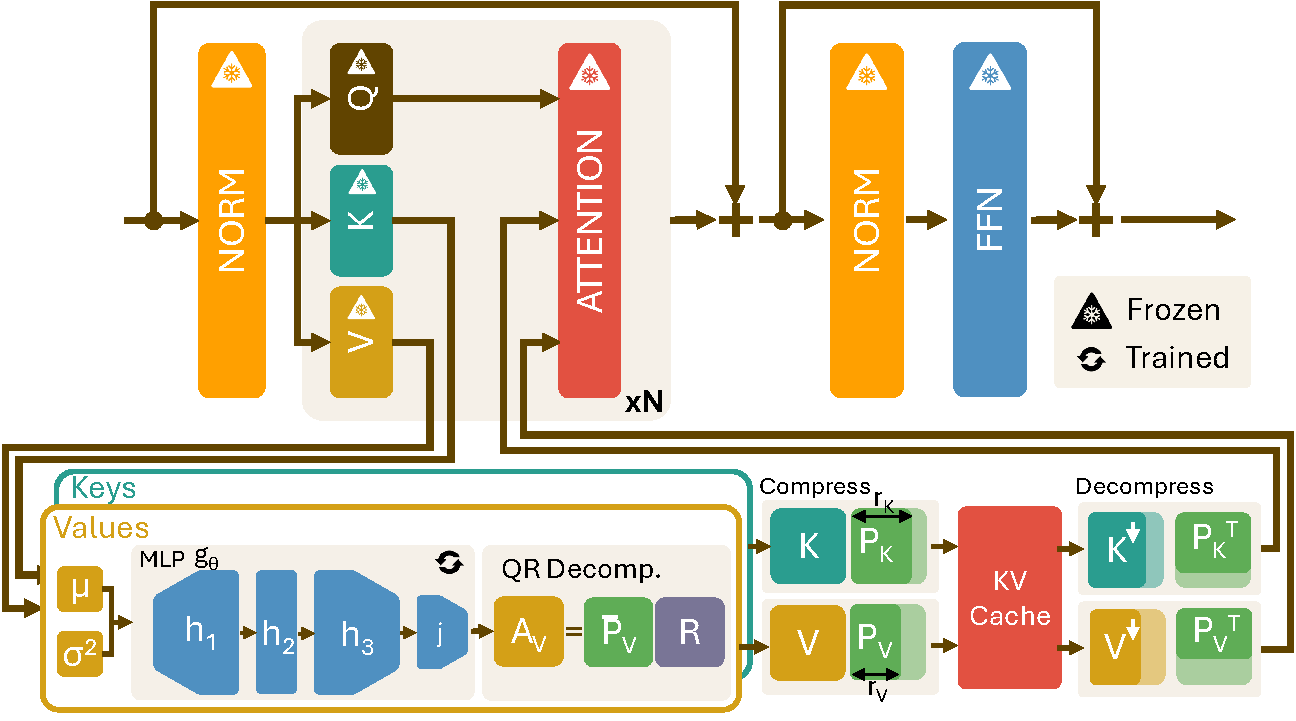
\includegraphics[width=\linewidth]{images/stief_att.pdf}
    \caption{Overview of \methodname. From lightweight activation statistics $\mu_{K}, \mu_{V}$ and $\sigma_{K}^2, \sigma_{V}^2$, we learn orthonormal projection bases $P_K, P_V$ which are optimized to minimize decoder-layer output error.}
    \label{fig:stief_att}
\end{figure}

\subsection{Goal}
SVD-like methods introduced in Sec.~\ref{subsec:backg_svdkvc} optimize proxy objectives on intermediate quantities (e.g., $K$, $[K;Q]$, or $QK^\top$).
In contrast, \methodname learns low-rank KV projections that directly minimize \emph{full decoder layer output} error.
Fig.~\ref{fig:stief_att} summarizes the core idea: instead of optimizing reconstruction in KV space, we optimize the error measured at the decoder-layer output, capturing the effect of both softmax and value mixing, as well as downstream transformations in the decoder layer, which includes output projection, residual paths, normalization and the MLP.

\subsection{Problem statement}
For each decoder layer $\ell$, let $f_\ell$ denote the original layer mapping and let $\tilde{f}_\ell$ denote the layer where keys and values inside attention are replaced by their reconstructed low-rank forms.
\methodname learns the $\bar P_K\in\mathbb{R}^{d_h\times d_h}$ and $\bar P_V\in\mathbb{R}^{d_h\times d_h}$ \emph{orthonormal projection bases}, and uses their leading $r_K, r_V \ll d_h$ columns to define the corresponding low-rank projection matrices:
\begin{equation}
\begin{aligned}
&P_K^{(r_K)} \coloneq \bar P_K[:,1{:}r_K]\in\mathbb{R}^{d_h\times r_K},\\
&P_V^{(r_V)} \coloneq \bar P_V[:,1{:}r_V]\in\mathbb{R}^{d_h\times r_V},
\end{aligned}
\label{eq:dkv_trunc_def}
\end{equation}
with $(P_K^{(r_K)})^\top P_K^{(r_K)} = I_{r_K}$ and $(P_V^{(r_V)})^\top P_V^{(r_V)} = I_{r_V}$.

Given full-precision matrices $K,V\in\mathbb{R}^{n\times d_h}$ (as obtained during calibration, or before compression is applied), \methodname forms and caches the compressed tensors
$K^{\downarrow}=K P_K^{(r_K)}$ and $V^{\downarrow}=V P_V^{(r_V)}$.
Whenever the attention block needs $K$ and $V$ in the original dimension, it uses the reconstructed forms:
\begin{equation}
\begin{aligned}
&\tilde K = K^{\downarrow}(P_K^{(r_K)})^\top = K P_K^{(r_K)}(P_K^{(r_K)})^\top,\\
&\tilde V = V^{\downarrow}(P_V^{(r_V)})^\top = V P_V^{(r_V)}(P_V^{(r_V)})^\top.
\end{aligned}
\label{eq:dkv_reconstruct}
\end{equation}

Given a set of calibration inputs $x$, \methodname finds $P_K$ and $P_V$ by solving through gradient descent the optimization problem:
\begin{equation}
\min_{\theta}\;\; \Delta_\ell(r_K,r_V;\theta;x),
\label{eq:dkv_obj}
\end{equation}
where $\Delta_\ell(r_K,r_V;\theta;x)$ denotes the relative error at the decoder-layer output:
\begin{equation}
\small
\Delta_\ell(r_K,r_V;\theta;x)
=
\mathbb{E}_{x}\!\left[
\frac{\| f_\ell(x) - \tilde{f}_\ell(x; r_K,r_V,\theta) \|_F}{\| f_\ell(x) \|_F}
\right],
\label{eq:dkv_delta}
\end{equation}
and $\theta$ parameterizes the predictor from which the projection bases $(P_K,P_V)$ are derived, described in the next Sec.~\ref{subsec:methods_basis_prediction}.

\subsection{Gradient-based basis prediction}
\label{subsec:methods_basis_prediction}
\methodname computes the $P_K, P_V$ orthonormal projection bases from simple activation statistics.
Let $K_x$ denote a collection of key vectors for layer $\ell$ computed over calibration samples $x$ and previously cached tokens.
We compute per-dimension mean and variance:
\begin{equation}
\begin{aligned}
&\mu_K = \mathbb{E}[K_x] \in \mathbb{R}^{d_h},\\
&\sigma_K^2 = \mathbb{E}\!\left[(K_x-\mu_K)^2\right] \in \mathbb{R}^{d_h},
\end{aligned}
\label{eq:dkv_stats}
\end{equation}
which are aggregated to form features $s_K=[\mu_K;\sigma_K^2]\in\mathbb{R}^{2d_h}$.
The same computation is performed to compute $s_V$ features over $V$ vectors.
Intuitively, $s_K$ and $s_V$ provide a cheap summary of first/second-order activation statistics from which the projection bases are computed, as will be described in subsequent paragraphs.
%
\paragraph{MLP architecture.}
We define a trainable predictor $g_\theta$ based on the MLP architecture depicted in the bottom part of Fig.~\ref{fig:stief_att}. The same architecture is employed for both keys and values. The predictor $g_\theta$ is trained by solving through gradient descent the optimization problem of Eq.~\ref{eq:dkv_obj}, to map the $s_K$ and $s_V$ statistics to $A_K$ and $A_V$ matrices whose orthonormalization and rank approximation yield a basis that minimizes decoder-layer output error.
%

Concretely, $g_\theta$ is an MLP composed of three hidden layers $h_i$ followed by a linear head $j$ that outputs the pre-orthonormalization matrix $A \in \mathbb{R}^{d_h\times d_h}$.
Let $s\in\mathbb{R}^{2d_h}$ denote the input feature vector (i.e., $s=s_K \: \text{or} \: s_V$).
%Writing two representative hidden layers explicitly,
The general form of hidden layers $h_i$ is:
\begin{equation}
h_i = \phi \left( \mathrm{LN}\left(W_i h_{i-1} + b_i\right) \right) \ \text{with} \ i \in \left[1, 3\right]
\label{eq:dkv_mlp}
\end{equation}
where $h_0 \equiv s$, $W_i$ and $b_i$ are the learnable weights and biases generically denoted as $\theta$ in Eq.~\ref{eq:dkv_obj} and Eq.~\ref{eq:dkv_delta}. $\phi(\cdot)$ is the GELU non-linearity and $\mathrm{LN}$ denotes LayerNorm.
While the final linear head producing $A$ is simply $j = W_j h_2 + b_j$.
%
We finally define:
%\begin{equation}
%A_K = g_{\theta}(s_K),\qquad A_V = g_{\theta}(s_V).
%\label{eq:dkv_raw}
%\end{equation}
\begin{equation}
A_K = g_{\theta_K}(s_K),\qquad A_V = g_{\theta_V}(s_V).
\label{eq:dkv_raw}
\end{equation}
where $\theta_K$ and $\theta_V$ respectively define the set of trainable parameters $\theta$ specific for the separate Key and Value predictors.

\paragraph{Orthonormalization via QR.}
We orthonormalize $A_K$ and $A_V$ via QR decomposition~\cite{bookqr}:
\begin{equation}
A_K = Q_K R_K,\qquad A_V = Q_V R_V,
\label{eq:dkv_qr}
\end{equation}
where $Q_K,Q_V\in\mathbb{R}^{d_h\times d_h}$ are matrices with orthonormal columns and $R_K,R_V$ are upper-triangular.\footnote{Here $Q$ does not denote the query vectors of Eq.~\ref{eq:bg_attn}.}
In \methodname, we use only the orthonormal factor $Q$, because our compression/reconstruction depends on the orthogonal projector $P P^\top$, which is determined solely by the subspace spanned by the columns of $P$.
Since $A$ and $Q$ span the same column space in a QR factorization, $Q Q^\top$ projects onto the same subspace as $A$.
The triangular factor $R$ only encodes a change of coordinates (and scaling) within that subspace and is therefore irrelevant for defining the projection basis.
Thus we set:
\begin{equation}
\bar{P}_K \coloneq Q_K,
\qquad
\bar{P}_V \coloneq Q_V.
\label{eq:dkv_bases}
\end{equation}
Ranks dimension is then applied by truncation as in Eq.~\ref{eq:dkv_trunc_def}.
%
%
%
%
\paragraph{Head sharing.}\label{par:head_sharing}
%\methodname uses different sharing schemes depending on the attention setting.
% In standard MHA, each attention head has its own $K,V$ cache, but we \emph{learn} one shared basis per layer for keys and one shared basis per layer for values (replicated across heads) to keep the predictor lightweight.
\methodname stores the cache per KV head.
We keep a single shared key basis per layer (i.e., one $\bar P_K$) and share it across KV heads, while we learn value bases per KV head: each head $h$ has $\bar P_{V,h}$ and its truncation $P_{V,h}^{(r_V)}$.
This choice provides a trade-off between overhead and flexibility, and reflects that keys are reused across multiple query heads in a group, while values interact with head-specific output-projection pathways.
%
\subsection{Training protocol}
% Alg.~\ref{alg:stiefattention} presents the \methodname training procedure of basis predictors $g_{\theta_V}, g_{\theta_K}$. 
% Crucially, training is performed along \emph{rank-conditioned propagation paths}: for each rank $r$ we maintain a propagated calibration stream $\{\mathcal{X}_V^{(\ell,r)}\}_{\ell \in \mathcal{L}}$ with initialization $\mathcal{X}_V^{(0,r)} = \mathcal{X}$.
% At layer $\ell$, we compute the activations $\mathcal{Z}^{(\ell,r)} = f_\ell\!\big(\mathcal{X}_V^{(\ell-1,r)}\big)$ and train $g_{\theta}(\ell,r,\mathcal{Z}^{(\ell,r)},\mathcal{E})$ via gradient descent to solve Eq.~\ref{eq:dkv_obj}, for keys and values independently.
% We then propagate the same-rank compressed forward pass by setting $\mathcal{X}^{(\ell,r)} = \tilde f_\ell^{(r)}\!\big(\mathcal{X}^{(\ell-1,r)}\big)$.
% This ensures that, for each rank $r$ we want to train, the predictors at deeper layers are trained on activations that already include the approximation error accumulated from earlier layers, capturing distribution shift and error compounding.
Alg.~\ref{alg:stiefattention} summarizes the \methodname training procedure for the basis predictors $g_{\theta_K}, g_{\theta_V}$ for keys and values.
We train each layer independently by calibrating layer $\ell$ on its uncompressed input activations $\mathcal{X}^{(\ell)}$.
Specifically, for each candidate rank, we train keys and values projection predictors $g_{\theta_K}, g_{\theta_V}$ independently by minimizing the relative decoder-layer output error of Eq.~\ref{eq:dkv_obj}.
We train bases following the head-sharing scheme above.
% for values, all per-KV-head bases at fixed $(\ell,r_V)$ are optimized jointly in a single run.

Finally, for each layer we evaluate $\Delta_\ell(r_K,r_V)$ over all candidate rank pairs $r_K \in \mathcal{R}_K$ and $r_V\in \mathcal{R}_V$ and store the resulting layer-wise error surface, which is later used for rank allocation (Sec.~\ref{sec:rank_selection}).


% \begin{algorithm}[t]
% \caption{\methodname basis predictor training}
% \label{alg:stiefattention}
% %\begin{algorithmic}[1]
% %{\renewcommand{\algorithmicrequire}{\textbf{Input:}}%
% %\REQUIRE Decoder layers $\mathcal{L}$; calibration set $\mathcal{X}$;
% %candidate ranks $\mathcal{R}_V$; epochs $\mathcal{E}$}
% %
% %\STATE \textbf{Propagated calibration set:} $\mathcal{X}_V^{(0)} \gets \mathcal{X}$
% %
% %\FOR{$\ell \in \mathcal{L}$}
% %  \FOR{$r \in \mathcal{R}_V$}
% %    \STATE $\mathcal{X}_{V}^{(\ell-1, r)} \gets \mathcal{X}_V^{(\ell-1)}$
% %    \STATE $\mathbf{Z}_V \gets f_{\ell}\!\left(\mathcal{X}_{V}^{(\ell-1, r)}\right)$
% %    \STATE $\mathrm{Train}\; g_{\theta_V}(\ell, r, \mathbf{Z}_V, \mathcal{E})$ to solve Eq.~\ref{eq:dkv_obj}
% %    \STATE $\mathcal{X}_{V}^{(\ell, r)} \gets \tilde f_{\ell}^{(r)}\!\left(\mathcal{X}_{V}^{(\ell-1, r)}\right)$
% %  \ENDFOR
% %\ENDFOR
% %
% %\STATE \textbf{Keys:} repeat Lines 1--9 replacing
% %$\mathcal{R}_V, g_{\theta_V}, \mathcal{X}_V$
% %with $\mathcal{R}_K, g_{\theta_K}, \mathcal{X}_K$.
% %\end{algorithmic}
% \begin{algorithmic}[1]
% {\renewcommand{\algorithmicrequire}{\textbf{Input:}}%
% \REQUIRE Decoder layers $\mathcal{L}$; calibration set $\mathcal{X}$;
% candidate ranks $\mathcal{R}_V$; epochs $\mathcal{E}$.}
% \FOR{$r \in \mathcal{R}_V$}
%   \STATE \textbf{Rank-conditioned propagated set:} $\mathcal{X}_V^{(0,r)} \gets \mathcal{X}$
%   \FOR{$\ell \in \mathcal{L}$}
%     \STATE $\mathcal{Z}_V^{(\ell,r)} \gets f_{\ell}\!\left(\mathcal{X}_V^{(\ell-1,r)}\right)$
%     \STATE $\mathrm{Train}\; g_{\theta_V}(\ell,r,\mathcal{Z}_V^{(\ell,r)},\mathcal{E})$ \COMMENT{solve Eq.~\ref{eq:dkv_obj}}
%     \STATE $\mathcal{X}_V^{(\ell,r)} \gets \tilde f_{\ell}^{(r)}\!\left(\mathcal{X}_V^{(\ell-1,r)}\right)$
%   \ENDFOR
% \ENDFOR
% \STATE \textbf{Keys:} repeat line 1-8 replacing $\mathcal{R}_V, g_{\theta_V}, \mathcal{X}_V, \mathcal{Z}_V$ with $\mathcal{R}_K, g_{\theta_K}, \mathcal{X}_K, \mathcal{Z}_K$.
% \end{algorithmic}
% \end{algorithm}
\begin{algorithm}[t]
\caption{\methodname basis training and error-surface construction}
\label{alg:stiefattention}
\begin{algorithmic}[1]
{\renewcommand{\algorithmicrequire}{\textbf{Input:}}%
\REQUIRE Decoder layers $\mathcal{L}$; calibration set $\mathcal{X}$; candidate ranks $\mathcal{R}_K,\mathcal{R}_V$.}
{\renewcommand{\algorithmicensure}{\textbf{Output:}}%
\ENSURE Key bases $\{\bar P_K^{(\ell,r_K)}\}_{\ell,r_K}$, value bases $\{\bar P_{V,h}^{(\ell,r_V)}\}_{\ell,r_V,h}$, error surfaces $\{\Delta_\ell(r_K,r_V)\}_{\ell,r_K,r_V}$.}

\FOR{$\ell \in \mathcal{L}$}
\STATE Forward pass on $\mathcal{X}$ and record $\mathcal{X}^{(\ell)}$.
    \FOR{$r_K \in \mathcal{R}_K$}
        \STATE Train $g_{\theta_K}^{(\ell,r_K)}$ on $\mathcal{X}^{(\ell)}$ to solve Eq.~\ref{eq:dkv_obj}
        \STATE Obtain $\bar P_K^{(\ell,r_K)}$ and truncated $P_K^{(\ell,r_K)}$
    \ENDFOR

    \FOR{$r_V \in \mathcal{R}_V$}
        \STATE Train $\{g_{\theta_{V,h}}^{(\ell,r_V)}\}_{h=1}^{H_{\mathrm{KV}}}$ \emph{jointly} on $\mathcal{X}^{(\ell)}$ to solve Eq.~\ref{eq:dkv_obj}
        \STATE Obtain $\{\bar P_{V,h}^{(\ell,r_V)}\}_{h=1}^{H_{\mathrm{KV}}}$ and truncated $\{P_{V,h}^{(\ell,r_V)}\}$
    \ENDFOR

    \FOR{$(r_K,r_V)\in\mathcal{R}_K\times\mathcal{R}_V$}
        \STATE Evaluate $\Delta_\ell(r_K,r_V)$ on $\mathcal{X}^{(\ell)}$ using $P_K^{(\ell,r_K)}$ and $\{P_{V,h}^{(\ell,r_V)}\}_{h=1}^{H_{\mathrm{KV}}}$
    \ENDFOR
\ENDFOR
\end{algorithmic}
\end{algorithm}
%
\subsection{Grid search and rank selection}
\label{sec:rank_selection}
% \methodname separates basis learning from rank selection by pre-computing a layer-wise error surface over the sets of candidate ranks $\mathcal{R}_K$ and $\mathcal{R}_V$.
% For each layer, we evaluate the error metric introduced in Eq.~\ref{eq:dkv_delta} for each $r_K\in\mathcal{R}_K$ and $r_V\in\mathcal{R}_V$.

% \ab{chiamerei il per-layer error budget $\epsilon_\ell$. Poi per le strategies in cui è sempre uguale metti $\epsilon_\ell = \epsilon \forall \ell$} \luca{io lascerei cosi, al massimo toglierei solo il "per-layer" se è misleading, ma l'error budget non è deciso per layer, è uno per tutto il modello.}
% Given a per-layer error budget
Given an error budget $\epsilon$, we evaluate different layer-wise rank-allocation policies that select $(r_K,r_V)$ using the precomputed error surface $\Delta_\ell(r_K,r_V)$ %$(obtained as an output of Alg. \ref{alg:stiefattention}).
A practical benefit of storing $\Delta_\ell$ is that rank allocation can be changed at model-deployment time \emph{without retraining bases}, providing an explicit accuracy--memory knob for different deployment constraints.
We evaluate the following selection policies:
\begin{enumerate}
    \item \textbf{Uniform:} use fixed ranks $(r_K, r_V)$ for all layers as a simple baseline;
    \item \textbf{Pareto:} for each layer, restrict candidates to the Pareto-optimal set of $(\Delta_\ell(r_K,r_V),\, r_K{+}r_V)$ pairs (i.e., no other candidate has both lower error and lower total rank), then choose among Pareto points the configuration with minimum $r_K{+}r_V$ subject to $\Delta_\ell(r_K,r_V)\le\epsilon$
    % (i.e., falling back to the minimum-error Pareto point if none satisfy the budget);
    \item \textbf{Weighted Pareto:} use a layer-dependent budget $\epsilon_\ell=\epsilon/w_\ell$, where $w_\ell$ is a fixed layer-sensitivity weight (a positional prior) that allocates tighter budgets to empirically fragile layers.
    Concretely, we set $w_\ell>1$ for the first and last four layers using a linear ramp ($2.0$ for first and last layers, 1.75, 1.5, 1.25 for the others in ascending/descending order) and $w_\ell=1$ elsewhere, then normalize $\{w_\ell\}_{\ell=1}^L$ to have mean $1$.
    Thus larger $w_\ell$ implies a smaller allowable error $\epsilon_\ell$ and typically higher selected ranks in those layers~\cite{li2025kvtuner,ma2023llmpruner}.
\end{enumerate}

\paragraph{Overheads.}
Importantly, the MLPs $g_\theta$ of Fig. 1 are only employed offline to learn projection bases, and the latter are the only extra parameters added to the model after calibration. Moreover, as in EigenAttention, projections can be folded into the attention linear weights~\cite{saxena2024eigenattention}. Thus, at inference time, \methodname incurs per-layer FLOP count and runtime data movement overheads identical to those of EigenAttention at iso-rank. 

% \subsection{Inference-time construction}
% \matteo{this is what eigen also does, so double check}
% \methodname uses the caching/reconstruction scheme from Sec.~\ref{sec:background} (Eqs.~\ref{eq:bg_compress}--\ref{eq:bg_reconstruct}).
% In practice we fold the down-projections into the linear weights:
% \begin{equation}
% W_{K}^{\downarrow} = W_K U_K^{(r_K)},
% \qquad
% W_{V}^{\downarrow} = W_V U_V^{(r_V)}.
% \label{eq:dkv_fold_kv}
% \end{equation}
% For values, the corresponding up-projection $(U_V^{(r_V)})^\top$ is applied after value mixing and can be absorbed into the per-head output projection blocks of $W_O$.
% If a layer selects full rank, we use identity projections and keep original weights to avoid overhead.

% \subsection{Inference-time construction} #short version
% \methodname uses the caching/reconstruction scheme from Sec.~\ref{sec:background} (Eqs.~\ref{eq:bg_compress}--\ref{eq:bg_reconstruct}).
% We follow the same weight-folding and inference construction used in prior projection-based methods (e.g., EigenAttention), and therefore omit further details.
